\section{Experiments}
\label{sec:experiments}
\subsection{Monk Results}
For the MONKS classification task we used a neural network with 17 input units, since we adopted the one-hot encoding, 5 nodes in the hidden layer and one for the output layer. The activation function we used in the layer was \textit{LeakyReLu}, meanwhile for the output layer we used the \textit{Sigmoidal} with its parameter $\alpha=1$. After many trials, with both mini-batch and batch gradient descent, we choose the latter since it made the loss functions curve smoother. The Tikhonov regularization was only used for \textit{MONK3} dataset because there was clearly a case of overfitting.
%Per il problema di classificazione riguardante i monks, è stata utilizzata una rete neurale con 17 unità di input, in seguito dell'adozione della one-hot encoding ed una unità nell'out layer. La funzione di attivazione utilizzata nell'unico hidden layer è stata la \textit{LeakyReLU}, mentre per l'output layer abbiamo utilizzato la \textit{Sigmoidal} con $\alpha=1$. Dopo varie prove, sia con mini-batch gradient descent che con batch gradient descent, si è scelto di utilizzare quest'ultimo perchè faceva risultare le curve della loss function più smooth. Weight decay è stato utilizzato solo per il \textit{MONK 3} dato che abbiamo potuto osservare un caso di overfitting.

%In this subsection report only plots and tables, comment only if needed. \\
%\textcolor{red}{[*] Lack of results in this part invalidates the report.  Both for A and B prj.} \\
%Please report:
%\vspace{-0.4cm}\begin{itemize}
    %\setlength\itemsep{-0.5em}
    %\item[-] Performance (see Table \ref{tab:monk-table}) and learning curves (MSE and accuracy plots for the 3 MONK’s tasks, see Fig. 2 as an example filled with the plot for the MONK2)
    %\item[-] Used hyper-parameters
%\end{itemize}
%\vspace{-0.5cm}
\begin{center}
    \begin{table}[H]
        \centering
        \small
        %\begin{tabular}{|l|l|l|l|l|l|l|}
        \begin{tabular}{|c|c|c|c|c|c|c|}
        %\begin{tabular}{|C{3.95cm}C{3.95cm}C{3.95cm}C{3.95cm}C{3.95cm}C{3.95cm}C{3.95cm}|}
            \hline
            \textbf{Task} & \textbf{\#units} & \textbf{$\eta$} & \textbf{$\lambda$} & \textbf{$\alpha$} & \textbf{MSE(TR/TS)} & \textbf{Acc(TR/TS)}\\ \hline
            
            MONK1 & 5  & 0.7 & 0 & 0.75 &  $1.5\times 10^{-3}$ / $2.5\times 10^{-3}$ & 100{\%} / 100{\%}\\ \hline
            
            MONK2 & 5 & 0.9 & 0 & 0.75 & $1.44\times 10^{-4}$ / $1.77\times 10^{-4}$ & 100{\%} / 100{\%} \\ \hline
            
            MONK3 & 5 & 0.8 & 0 & 0.85 & $1.45\times 10^{-2}$ / $5.5\times 10^{-2}$ & 97.21{\%} / 93.94{\%} \\ \hline
            
            MONK3+reg. & 5 & 0.8 & 0.01 & 0.85 & $4.1\times 10^{-2}$ / $3.5\times 10^{-2}$ & 95.41{\%} / 97.03{\%} \\ 
            
            \hline
        \end{tabular}
        \caption{Average prediction results obtained for the MONK’s tasks.}
        \label{tab:monk-table}
    \end{table}
\end{center}
\begin{figure}[H]%
    \centering
    %\hfill
    \subfloat[MSE MONK1]{{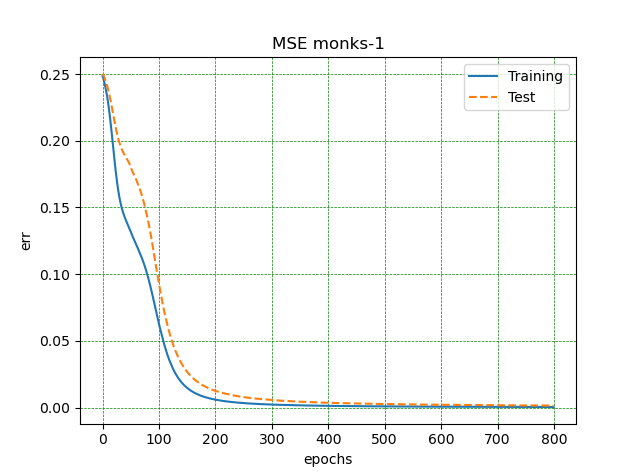
\includegraphics[width=0.50\linewidth]{Figure/Monk/monk1mse.png}}}%
    %\qquad
    %\hfill
    \subfloat[Accuracy MONK1]{{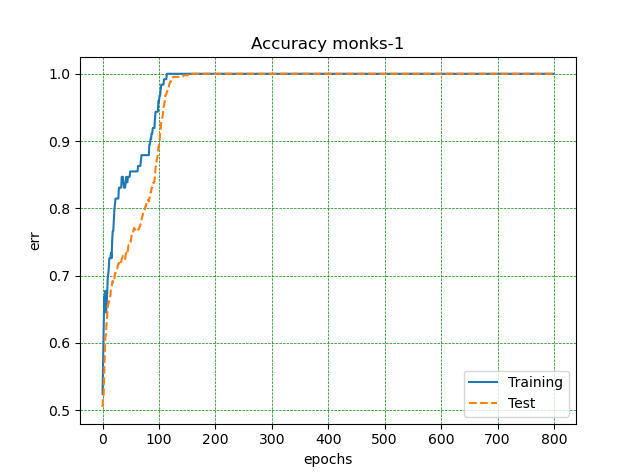
\includegraphics[width=0.50\linewidth]{Figure/Monk/monk1acc.png}}}%
    %\hfill
    %\caption{Il problema del commesso viaggiatore, immagine trovata dal web}
    %\caption{Rappresentazione degli archi del grafo basato sul sudoku}
    %\caption{Articoli per anno contenenti "Genetic Algorithm", fonte dei dati: Google Scholar}
    \caption{MSE and accuracy for MONK1}
    \label{fig:monk1}%
\end{figure}
\begin{figure}[H]%
    \centering
    %\hfill
    \subfloat[MSE MONK2]{{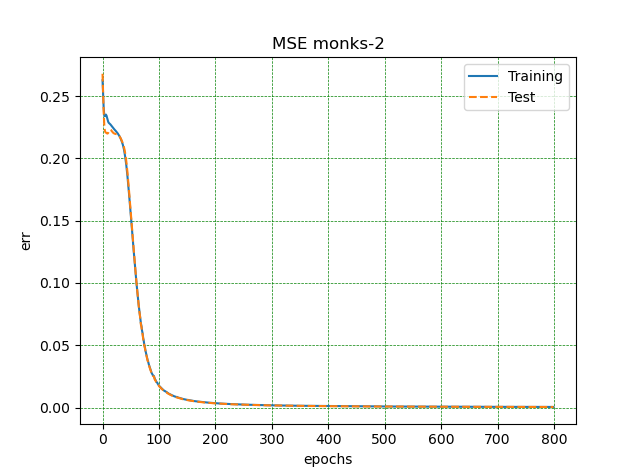
\includegraphics[width=0.50\linewidth]{Figure/Monk/monk2mse.png}}}%
    %\qquad
    %\hfill
    \subfloat[Accuracy MONK2]{{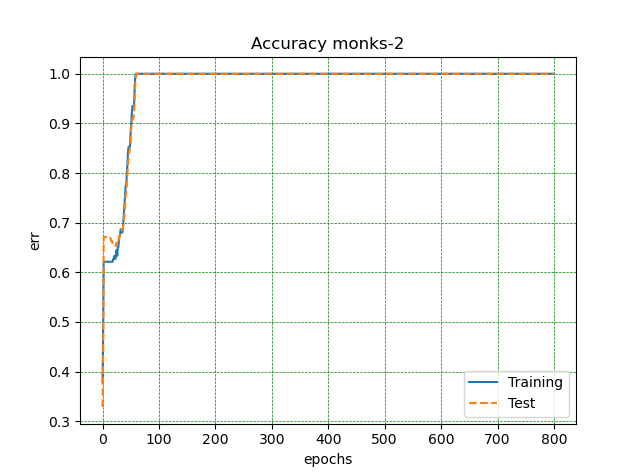
\includegraphics[width=0.50\linewidth]{Figure/Monk/monk2acc.png}}}%
    %\hfill
    %\caption{Il problema del commesso viaggiatore, immagine trovata dal web}
    %\caption{Rappresentazione degli archi del grafo basato sul sudoku}
    %\caption{Articoli per anno contenenti "Genetic Algorithm", fonte dei dati: Google Scholar}
    \caption{MSE and accuracy for MONK2}
    \label{fig:monk2}%
\end{figure}
\begin{figure}[H]%
    \centering
    %\hfill
    \subfloat[MSE MONK3]{{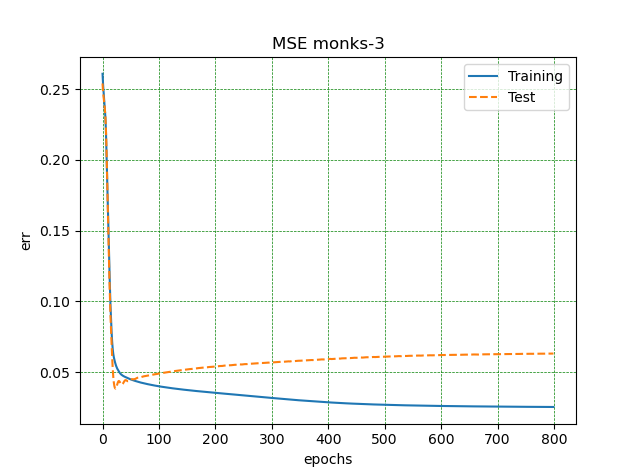
\includegraphics[width=0.50\linewidth]{Figure/Monk/Figure_1.png}}}%
    %\qquad
    %\hfill
    \subfloat[Accuracy MONK3]{{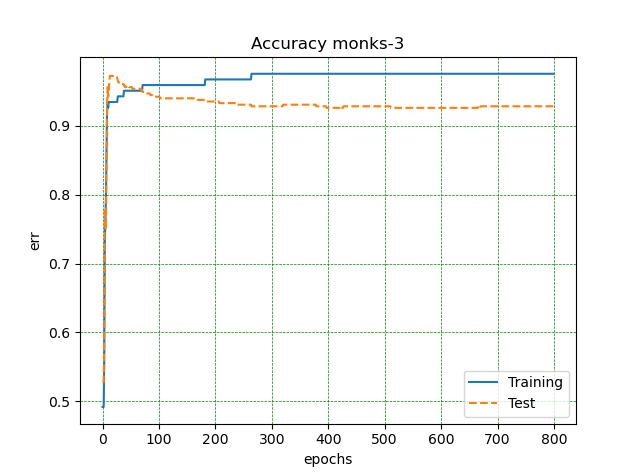
\includegraphics[width=0.50\linewidth]{Figure/Monk/Figure_2.png}}}%
    %\hfill
    %\caption{Il problema del commesso viaggiatore, immagine trovata dal web}
    %\caption{Rappresentazione degli archi del grafo basato sul sudoku}
    %\caption{Articoli per anno contenenti "Genetic Algorithm", fonte dei dati: Google Scholar}
    \caption{MSE and accuracy for MONK3}
    \label{fig:monk3}%
\end{figure}
\begin{figure}[H]%
    \centering
    %\hfill
    \subfloat[MSE MONK3+reg]{{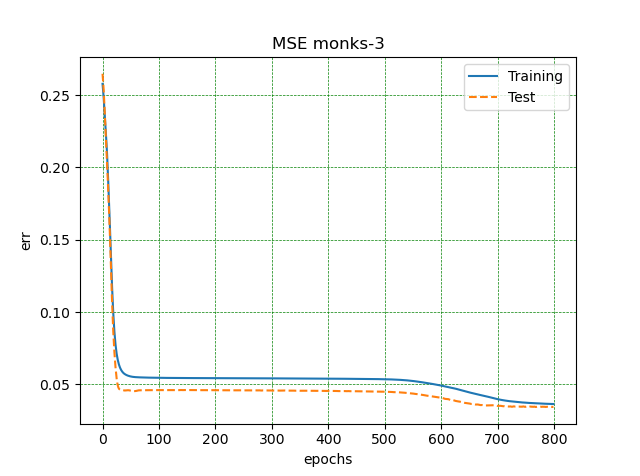
\includegraphics[width=0.50\linewidth]{Figure/Monk/monk3mse_reg.png}}}%
    %\qquad
    %\hfill
    \subfloat[Accuracy MONK3+reg]{{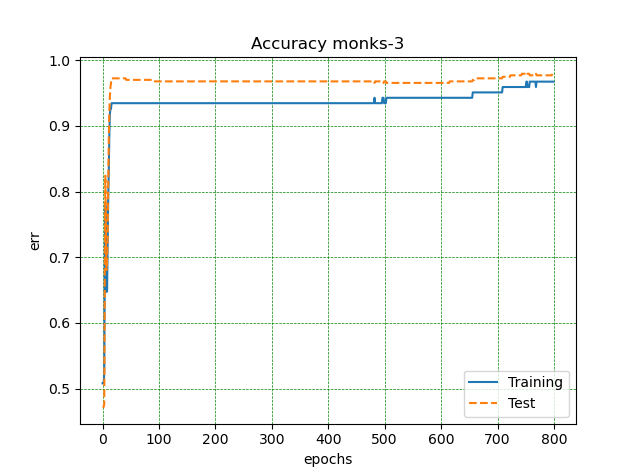
\includegraphics[width=0.50\linewidth]{Figure/Monk/monk3acc_reg.png}}}%
    %\hfill
    %\caption{Il problema del commesso viaggiatore, immagine trovata dal web}
    %\caption{Rappresentazione degli archi del grafo basato sul sudoku}
    %\caption{Articoli per anno contenenti "Genetic Algorithm", fonte dei dati: Google Scholar}
    \caption{MSE and accuracy for MONK3+reg}
    \label{fig:monk3reg}%
\end{figure}
For each MONK dataset we showed only one plot for the MSE and the accuracy since all the plot were very similar between each other: the curves on MONK1 and MONK2 converged a little before the 300 epochs, meanwhile for the MONK3 we needed about 500 epochs in its no regularized form and more than 750 for the regularized one. Anyway, we decided to show only the first 800 epochs for each dataset since there wasn't any major improvement over the learning curves.
%\newpage
\subsection{Cup Results}
\label{subsec:cupResult}
\subsubsection{Validation}
Talking about the validation phase, we have chosen to partition the ML-CUP20-TR dataset in order to obtain an 80{\%} for development and the remaining 20{\%} for internal testing. In order to select the best model, we have chosen to apply the K-Fold cross validation, with 4 folds, for each combination of hyperparameters of the grid search. The choice of k was made taking into account the execution time of the validation phase and preserving a correct balance of data in the training set and in the validation set.

%Per la fase di validation, si è scelto di partzionare il data set ML-CUP20-TR così da ottenere 80{\%} per il training e il restante 20{\%} per il test interno. Per la selezione del modello migliore, abbiamo scelto di applicare la K-Fold cross validation, con 4 folds, per ogni combinazione di hyperparameters derivante dalla grid search. La scelta di k è stata fatta tenendo conto del tempo di esecuzione della fase di validation e per preservare un giusto bilanciamento del training set e del validation set.

\subsubsection{Screening phase}\label{subsubsec:screeningPhase}
The initial approach was to create two neural networks, which differ only in the activation function of the hidden layer: the first with \textit{TanH}, while the second with \textit{LeakyReLU}, both with only one hidden layer with 30 units and two nodes in the out layer with \textit{Linear} activation function. Then we applied k-fold cross validation with grid search and we observed that the first network was characterized by a smoother learning curve and a lower validation error than the second one. Adding nodes or a hidden layer always produced better behavior for the network with \textit{TanH}. We then repeated the procedure comparing \textit{TanH} and \textit{Sigmoid}. We noticed that the behaviour of the learning curves was very similar, but the \textit{TanH}, in the same configuration, produced a lower error in the validation set. Understood that, we continued the hyperparameters tuning phase using this activation function (\textit{TanH}) and with the batch approach since it didn't add noise to our learning curves.
%L'approccio iniziale è stato quello di creare due reti rete neurali, che differiscono solo per la funzione di attivazione nell'hidden layer: la prima con \textit{TanH}, mentre la seconda con \textit{LeakyReLU} ed entrambe con un solo hidden layer con 15 unità e due nodi nell'out layer con funzione di attivazione \textit{Linear}. Si è poi applicata la cross validation con grid search e si è osservato come la prima rete fosse caratterizzata da una curva di apprendimento più smooth che si traduceva in un errore sul validation set minore della seconda. L'aggiunta di nodi o di un hidden layer produceva sempre un comportamento migliore per la rete con \textit{TanH}. Successivamente abbiamo ripetuto la procedura confrontando \textit{TanH} e \textit{Sigmoid}. Si è notato come il comportamento delle curve di apprendimento fosse sovrapponibile, ma la \textit{TanH}, a parità di nodi, produceva un errore sul validation set minore. Capito ciò, abbiamo proseguito la ricerca dei migliori ipeparamentri utilizzando tale funzione di attivazione.

\subsubsection{Hyperparameters}\label{subsubsec:hyperparameters}
During the screening phase described in \ref{subsubsec:screeningPhase} we tried, for each hyperparameter, very large ranges: in particular, the learning rate $\eta \in [0.001, 0.03$ with step $0.002$, momentum $\alpha \in [0.3, 0.9]$ with step $0.1$, one hidden layer with \#nodes $in [15, 35, 60]$ and two hidden layers, respectively with [30, 40, 50] nodes. After this phase, we squeezed the ranges for each hyperparameter and we applied the grid-search with the aim to retrieve the best combinations. The table \ref{tab:hyperparam} shows the subsets on wich we applied the grid-search, for a total of 375 configurations; we then applied the internal test on the 10 best ones.
%Durante la screening phase descritta in \ref{subsubsec:screeningPhase} avevamo provato, per ogni iperparametro, dei range molto ampi: in particolare, il learning rate $\eta \in [0.001, 0.03]$ con passo $0.002$, momentum $\alpha \in [0.3, 0.9]$ con passo $0.1$, un hidden layer con \#nodi $\in [15, 35, 60]$ e due hidden layer, rispettivamente con [30, 40, 50] nodi. Terminata questa fase, ci siamo concentrati nei migliori sottoinsiemi per ciascun iperparametro. La tabella \ref{tab:hyperparam} mostra tali sottoinsiemi sui quali abbiamo eseguito la grid search, per un totale di 375 configurazioni. Sulle 10 migliori abbiamo poi eseguito il test interno.
\begin{center}
    \begin{table}[H]
        \centering
        \small
        %\begin{tabular}{|l|l|l|l|l|l|l|}
        \begin{tabular}{|c|c|}
        %\begin{tabular}{|C{3.95cm}C{3.95cm}C{3.95cm}C{3.95cm}C{3.95cm}C{3.95cm}C{3.95cm}|}
            \hline
            \textbf{Hyperparameter} & \textbf{Possible values} \\ \hline
            
            structure & $\{[30, 30], [40,30], [40, 40], [50, 40], [50, 50]\}$ \\ \hline
            
            $\alpha$ & [0.5, 0.6, 0.7, 0.8, 0.9] \\ \hline
            
            $\eta$ & [0.001, 0.003, 0.005, 0.007, 0.009] \\ \hline
            
            $\lambda$ & [0.00001, 0.00003, 0.00005] \\ \hline
            
            activation function (hidden) & TanH \\ \hline
            
            activation function (output) & Linear(1) \\ \hline
            
            batch size & full-batch \\
            
            \hline
        \end{tabular}
        \caption{The hyperparameters subranges on which we executed the grid-search.}
        \label{tab:hyperparam}
    \end{table}
\end{center}
\subsubsection{Best models}
As we said in \ref{subsubsec:hyperparameters}, we've taken the best 10 models from the 375 configurations and we applied the internal test on them, the table \ref{tab:bestmodels} shows the MEE on the training, validation and the internal test set.
\begin{center}
    \begin{table}[H]
        \centering
        \small
        %\begin{tabular}{|l|l|l|l|l|l|l|}
        \begin{tabular}{|c|c|c|c|c|c|c|c|}
        %\begin{tabular}{|C{3.95cm}C{3.95cm}C{3.95cm}C{3.95cm}C{3.95cm}C{3.95cm}C{3.95cm}|}
            \hline
            \textbf{Model} & \textbf{Structure} & $\alpha$ & $\eta$ & $\lambda$ & \textbf{MEE Tr} & \textbf{MEE Val} & \textbf{MEE Ts} \\ \hline
            
            0 & [50, 40] & 0.6 & 0.003 & 0.00003 & 2.7211 & 2.9747 & 2.8590 \\ \hline
            
            1 & [50, 40] & 0.6 & 0.003 & 0.00001 & 2.7544 & 2.9846 & 2.8679 \\ \hline
            
            2 & [50, 50] & 0.5 & 0.005 & 0.00001 & 2.6943 & 2.9915 & 2.8822 \\ \hline
            
            3 & [50, 50] & 0.6 & 0.003 & 0.00001 & 2.7381 & 2.9772 & 2.8609 \\ \hline
            
            4 & [30, 30] & 0.5 & 0.003 & 0.00003 & 2.7858 & 2.9845 & 2.9771 \\ \hline
            
            5 & [40, 40] & 0.5 & 0.003 & 0.00005 & 2.7937 & 2.9942 & 2.7577 \\ \hline
            
            6 & [40, 40] & 0.6 & 0.003 & 0.00003 & 2.7667 & 2.9936 & 2.9444 \\ \hline
            
            7 & [40, 40] & 0.6 & 0.005 & 0.00001 & 2.6731 & 2.9769 & 2.8504 \\ \hline
            
            8 & [50, 40] & 0.5 & 0.003 & 0.00001 & 2.7799 & 2.9891 & 2.9050 \\ \hline
            
            9 & [40, 30] & 0.5 & 0.003 & 0.00001 & 2.7611 & 2.9998 & 2.6899 \\ \hline
            
            \hline
        \end{tabular}
        \caption{MEE for the 10 best models obtained through the grid-search}
        \label{tab:bestmodels}
    \end{table}
\end{center}
We want to underline the fact that we obtained models with a training error smaller than the ones shown on table \ref{tab:bestmodels} (the range was [1.9, 2.3]), but their validation error was significantly higher and their plots showed a very clear case of overfitting, so we opted to taking in account only those that had the smallest validation error among the 375 configurations; we also noted that for $\alpha>0.6$ the validation error was never under the 3 threshold.
We computed the training and internal test with 3000 epochs for each best model and it took, on average, 390.859 seconds (6.51 minutes) on the following machines:
\begin{itemize}
    \item Intel i7-1065G7, 1.3GHz, 16GB RAM DDR4;
    \item AMD Ryzen 7 4800H 2.9GHz, 16GB RAM DDR4.
\end{itemize}
\subsubsection{Chosen model}
We chose the best model based, first of all, on the average results produced by each model on the validation set, in reference to the table \ref{tab:bestmodels} and as a second yardstick on the error in the internal test. The model that performed better was number 7, the one composed of two hidden layers with 40 nodes each, $\alpha = 0.6$, $\eta = 0.005$ and $\lambda = 0.00001$. As a result, we ran the CUP blind test using this model.

\begin{figure}[H]%
    \centering
    %\hfill
    \subfloat[MEE CUP]{{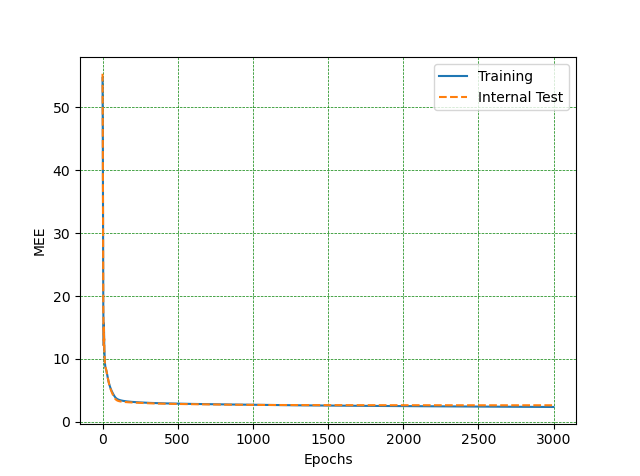
\includegraphics[width=0.50\linewidth]{Figure/Cup/chosen_model.png}}}%
    %\qquad
    %\hfill
    \subfloat[MEE CUP Zoom In]{{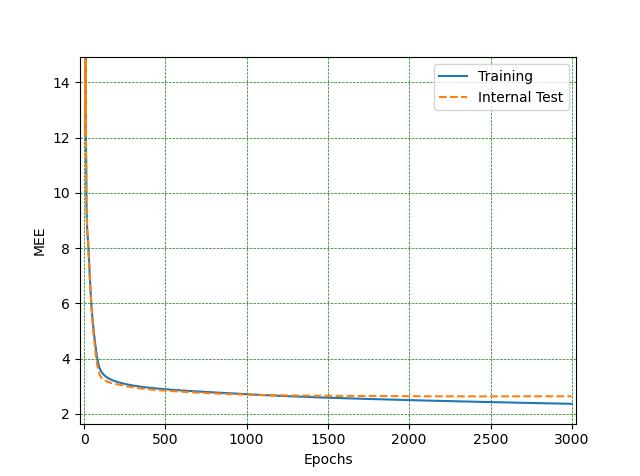
\includegraphics[width=0.50\linewidth]{Figure/Cup/chosen_model1.png}}}%
    %\hfill
    %\caption{Il problema del commesso viaggiatore, immagine trovata dal web}
    %\caption{Rappresentazione degli archi del grafo basato sul sudoku}
    %\caption{Articoli per anno contenenti "Genetic Algorithm", fonte dei dati: Google Scholar}
    \caption{MEE CUP internal test with chosen model.}
    \label{fig:cup}%
\end{figure}
Figure \ref{fig:cup} shows the plot of the training and internal test MEE by using model 7.
%\underline{\textbf{\textit{Always include:}}}
%\begin{enumerate}
    %\setlength\itemsep{-0.25em}
    %\item \underline{Details of the Validation schema} (model selection and assessment schema): Splitting  TR/VL/(internal)TS (\% data for each set and/or the K values of the k-fold CV)  \textcolor{red}{[*]}
    %\item Screening phase: Type of preliminary trials pursued (often summarized by text) 
    %\item Schema and \underline{range} of explored hyper-parameters (values used for the grid search, possibly a table) \textcolor{red}{[*]}
    %\item Grid search: \underline{TABLES of results} TR/VL/(TS)\textsuperscript{\textbf{\textcolor{red}{iii}}} with MEE \textcolor{red}{[*]}. At least the most performant cases. Tables/Plots can be used also to show some relevant trends for specific hyper-parameters changes (if you think it is significant) 
    %\item Provide an estimation of the (training) computing time (and of your HW resources)
    %\item Repeat and compare if you are comparing different models/algorithms/approaches (or different variants of the approach that you think are significant). 
    %\item \textbf{\textit{Define how you selected the}} \underline{FINAL model} used on the blind test set \textcolor{red}{[*]}. \underline{Which is it among the candidates and why?} Also write the  hyper-param. of the final model \textcolor{red}{[*]}.
    %\item \textbf{\textit{Report}} for the \underline{FINAL model} used on the blind test set the \underline{TABLE with MEE} for \underline{TR (training)}, \underline{VL (validation)} and \underline{TS (internal TS)}\textsuperscript{\textbf{\textcolor{red}{iv}}} \underline{in the original scale} \textcolor{red}{[*]}\textcolor{red}{[*]}. Note again  that you must have an internal  test evaluation (see the note IV above)
    %\item Plot the \underline{learning curve} TR/(VL)\textsuperscript{\textbf{\textcolor{red}{v}}}/TS for the FINAL model \textcolor{red}{[*]} (the final model is unique) 
    %\item Discussion (what you found more relevant in your experiments)
%\end{enumerate}
%\textcolor{red}{[*] = Lack of results in this part invalidates the report. Both for A and B prj.} \\
%\textbf{Further explanations and notes:} \\
%A good experimental report lists observed facts \textit{supported by experimental evidence}:
%\begin{itemize}
    %\setlength\itemsep{-0.25em}
    %\item[$\circ$] Report of used  setting (\textbf{\textit{replicability}}), and of the procedure for model selection and validation/assessment
    %\item[$\circ$] Report accurate results in numerical and graphical form (clear tables/plots with measures of training, validation and test errors)
    %\item[$\circ$] Make a selection of the evidences that you think are important but for those  show with graphs / tables etc, e.g. by plots varying the hyperparameters values
    %\item[$\circ$] Make critical remarks (+/-) on the effect of your choices (and, if necessary, their agreement with the theory of ML or report and discuss unusual evidences)
    %\item[$\circ$] Note that the relative position between the different cases is interesting (not the absolute performance)
    %\item[$\circ$] Learning curve to show the TR, Val/Test error with the progress of training: Curve with LMS (loss used for training) and measure of final error curve (e.g. accuracy for classification) can be different
%\end{itemize}